\documentclass[titlepage,oneside,final,14pt]{extarticle} % тип документа (титульник, односторонняя, финальная версия, 14 пункт по дефолту)

\usepackage[utf8]{inputenc} % кодировка
\usepackage[english,russian]{babel} % переносы и поддержка языка
\usepackage{indentfirst} % отступы в абзаце
\usepackage{vmargin}
\usepackage{hyperref} % гиперссылки
\usepackage{listings} % листинги кода
\usepackage{color} % создание цветов
\usepackage{graphicx} % картинки
\usepackage{tempora} % шрифт
\usepackage{float} % чтоб картинки не плавали [H]
\usepackage{setspace} 
\usepackage{chngcntr} 
\usepackage{ccaption} 
\usepackage{titlesec} % для заголовков
\usepackage{ragged2e} % для выравнивания по ширине
\usepackage{enumitem} % для межстрочного интервала в списках

\setlist{noitemsep} % убирает отступы для элементов списка
\titleformat{\section}[hang]{\normalfont\Large\bfseries\filcenter}{\thesection}{1em}{}[] % настройки заголовков
\titleformat{\subsection}[hang]{\filcenter\bfseries}{\thesubsection}{1em}{}[]
\titleformat{\subsubsection}[hang]{\filcenter\bfseries}{\thesubsubsection}{1em}{}[]
\newcommand{\sectionbreak}{\clearpage} % для разрыва листа для новой секции

\RequirePackage{caption}
\DeclareCaptionLabelSeparator{defis}{ --- }
\captionsetup{justification=centering,labelsep=defis} % для тире в подписях к картинкам

\counterwithin{figure}{section} % счетчик для картинок
\onehalfspacing % полуторный интервал
\graphicspath{{./images/}} % путь к папке с картинками
\setpapersize{A4} % а4 лист
\setmarginsrb{30mm}{20mm}{15mm}{20mm}{0pt}{0mm}{0pt}{10mm} % поля - левое, верхнее, правое, нижнее
\parindent=1.25cm % абзацный отступ
\sloppy % чтоб не вылезало за пределы листа
\lstset{language=Java,
	showspaces=false,
	showtabs=false,
	breaklines=true,
	showstringspaces=false,
	breakatwhitespace=true,
	commentstyle=\color{pgreen},
	keywordstyle=\color{pblue},
	stringstyle=\color{pred},
	basicstyle=\linespread{1}\small\ttfamily,
	columns=fullflexible
} % настройки листинга кода

\definecolor{pblue}{rgb}{0.13,0.13,1}
\definecolor{pgreen}{rgb}{0,0.5,0}
\definecolor{pred}{rgb}{0.9,0,0}
\definecolor{pgrey}{rgb}{0.46,0.45,0.48}

\hyphenpenalty=10000 % для отсутствия переносов
\justifying % по ширине

\author{Bulychev Ivan}
\title{Лабораторная работа №1}

\begin{document}
	
\begin{titlepage}
	\begin{spacing}{1.1}
		\begin{center}		
			ФЕДЕРАЛЬНОЕ АГЕНТСТВО СВЯЗИ 
			\\
			Федеральное государственное бюджетное образовательное учреждение высшего образования
			\\
			<<ПОВОЛЖСКИЙ ГОСУДАРСТВЕННЫЙ УНИВЕРСИТЕТ ТЕЛЕКОММУНИКАЦИЙ И ИНФОРМАТИКИ>>
			\\			
			\vspace{1em}
			Факультет информационных систем и технологий
			\\
			Кафедра программного обеспечения и управления в технических системах
			\\
			\vspace{7em}
			\bfseries\Large
			ОТЧЕТ
			\\
			ПО ЛАБОРАТОРНОЙ РАБОТЕ № \underline{\hspace{0.4em}1\hspace{0.4em}}
			\\
			\vspace{0.5em}
			\normalfont
			\normalsize
			по дисциплине
			\underline{\hspace{4em}Параллельное программирование\hspace{4em}}
			\\
			\small
			\hspace{4em} название (при наличии)
			\normalsize
			\\
			\hspace{3em}			
			\underline{\hspace{3em}Запуск консольного приложения на кластере MPI\hspace{3em}}
			\\
			\small
			\hspace{4em} название работы (при наличии)
			\normalsize
			\\		
	\end{center}			
			\vspace{5em}
			\begin{minipage}{0.5\textwidth}
				\begin{flushleft}					
				\end{flushleft}
			\end{minipage}
			\begin{minipage}{0.5\textwidth}
				\begin{center}
					\bfseries
					ВЫПОЛНИЛ
					\\
					\normalfont
					студент \hspace{1ex} \underline{гр. ПО--61} \hspace{1ex} \underline{Булычев И. Д.}
					\\
					\small
					\hspace{3.5em} (группа) \hspace{3.5em} (ФИО)
					\normalsize\bfseries
					ПРОВЕРИЛА
					\\
					\normalfont
					\hspace{1ex} \underline{к. т. н., доцент} \hspace{1ex} \underline{Мезенцева Е. М.}
					\\
					\small
					(должность) \hspace{5em} (ФИО)
					\\	
					\normalfont				
				\end{center}
			\end{minipage}
		\begin{center}
			\vspace{6em}
			Самара
			\\
			2019
			\end{center}

			

\end{spacing}
\end{titlepage}
\setcounter{page}{2}

\section{Цель лабораторной работы}

\subsection{Цель работы}

Необходимо реализовать программу, процессы которой обмениваются данными, введенными пользователем.

\subsection{Используемое программное обеспечение}

Для выполнения лабораторной работы мною было использовано следующее программное обеспечение:
\begin{itemize}
	\item ОС Ubuntu 18.10
	\item IDE Intellij Idea 2018.3
	\item JDK 1.8
	\item MPJ Express 0.44
\end{itemize}

\section{Результаты выполнения лабораторной работы}

\subsection{Содержимое файла input.txt}

\ttfamily

1

20

300

4000

0

9999999999


\normalfont

\begin{figure}[H]
	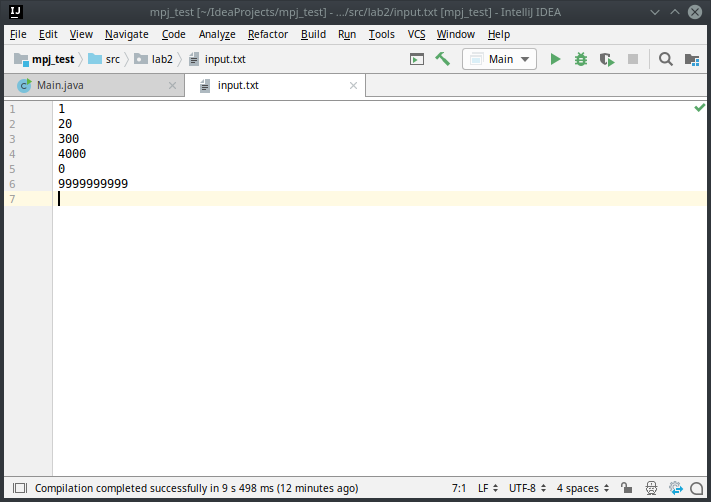
\includegraphics[width=1\linewidth]{input_txt}
	\centering
	\caption{Файл input.txt}
\end{figure}

\subsection{Листинг приложения}

\begin{lstlisting}

package lab2;

import mpi.MPI;

import java.io.File;
import java.util.Scanner;

public class Main {
  public static void main(String[] args) throws Exception {
    MPI.Init(args); // initialization
    Scanner in = new Scanner(new File("src/lab2/input.txt"));
    int[] num = new int[1]; //array creation
    // 0 - main process
    do {
      if (MPI.COMM_WORLD.Rank() == 0) {
        num[0] = in.nextInt(); // reading an int from file
      }
      MPI.COMM_WORLD.Bcast(num, 0, 1, MPI.INT, 0); // cast an array to all other processes
      System.out.println("hello from process " + MPI.COMM_WORLD.Rank() + ", num = " + num[0]);
    } while (num[0] != 0);
  System.out.println("input equals zero, shutting down process " + MPI.COMM_WORLD.Rank());
  MPI.Finalize();
  }
}


\end{lstlisting}

\subsection{Результат выполнения}
\ttfamily
hello from process 0, num = 1

hello from process 1, num = 1

hello from process 2, num = 1

hello from process 3, num = 1

hello from process 2, num = 20

hello from process 3, num = 20

hello from process 0, num = 20

hello from process 1, num = 20

hello from process 3, num = 300

hello from process 2, num = 300

hello from process 0, num = 300

hello from process 1, num = 300

hello from process 3, num = 4000

hello from process 2, num = 4000

hello from process 0, num = 4000

hello from process 1, num = 4000

hello from process 3, num = 0

input equals zero, shutting down process 3

hello from process 2, num = 0

input equals zero, shutting down process 2

hello from process 0, num = 0

input equals zero, shutting down process 0

hello from process 1, num = 0

input equals zero, shutting down process 1

\normalfont

\begin{figure}[H]
	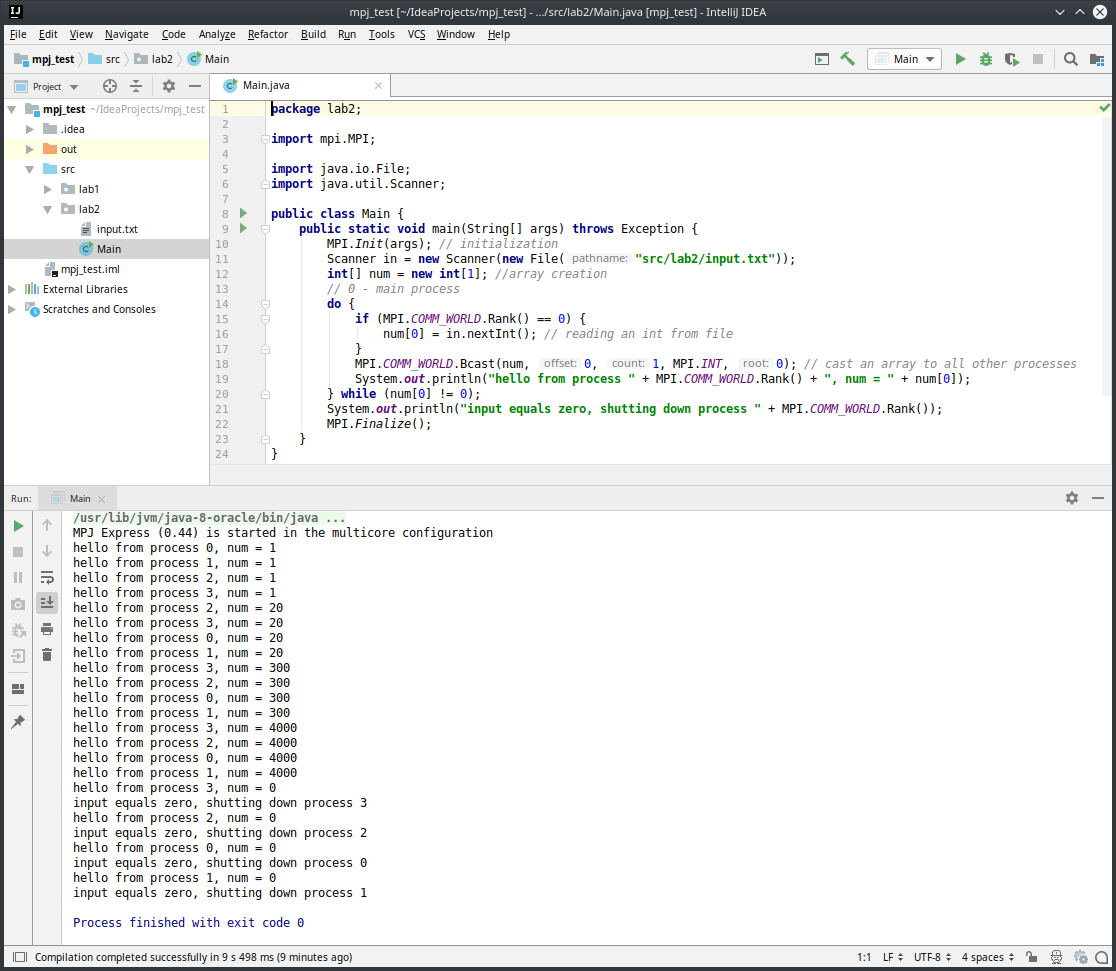
\includegraphics[width=1\linewidth]{code_listing_results}
	\centering
	\caption{Листинг и результат выполнения}
\end{figure}

\section{Выводы по результатам выполнения лабораторной работы}

В данной работе была написана программа, которая обеспечивает обмен данными между нулевым процессом и всеми остальными. Это делается с помощью MPI функции MPI\_Bcast. Нулевой процесс читает число из файла, после чего рассылает его всем процессам. После этого каждый процесс выводит на экран полученное сообщение с указанием своего номера. Процесс ввода продолжается до получения нуля.

\end{document}
